\documentclass[11pt]{article}

\usepackage[margin=1in]{geometry}
\usepackage{amsmath,amssymb,amsfonts}
\usepackage{mathtools}
\usepackage{bm}
\usepackage{booktabs}
\usepackage{multirow}
\usepackage{graphicx}
\usepackage{xcolor}
\usepackage{enumitem}
\usepackage[colorlinks,urlcolor=blue,linkcolor=blue,citecolor=blue]{hyperref}

\newcommand{\R}{\mathbb{R}}
\newcommand{\bF}{\mathbf{F}}
\newcommand{\bq}{\mathbf{q}}
\newcommand{\bu}{\mathbf{u}}
\newcommand{\bz}{\mathbf{z}}
\newcommand{\bmu}{\boldsymbol{\mu}}
\newcommand{\cK}{\mathcal{K}}
\newcommand{\cU}{\mathcal{U}}
\newcommand{\tobj}{\tau_{\text{obj}}}
\newcommand{\tabs}{\tau_{\text{abs}}}
\newcommand{\tens}{\tau_{\text{ens}}}
\DeclareMathOperator*{\argmin}{arg\,min}
\title{Supplementary Material for\\Structured Abstention Segmentation: Native Unknown Representation for Open-World Dense Prediction}
\author{}
\date{}

\begin{document}

\maketitle

\section{Additional Method Details}

This section collects implementation details that are secondary to the main conceptual
contributions of SASeg but are useful for reproducibility.

\subsection{Encoder and Pixel Decoder Details}

We adopt Swin Transformer Tiny (Swin-T, ImageNet-21k pre-trained) as the encoder,
producing four-scale feature maps at strides $\{4, 8, 16, 32\}$.
The first two stages are frozen during training, while the last two are fine-tuned at
$10^{-5}$ learning rate.
A standard FPN pixel decoder fuses these features into a dense feature map
$\bF \in \R^{\frac{H}{4} \times \frac{W}{4} \times 256}$ ($d=256$).
Boundary refinement is handled by the auxiliary boundary-suppression term rather than
additional decoder modules.

\subsection{Prototype Initialization and Update}

For the prototype-sphere support module, we use $R=2$ prototype-spheres per known
class in the default configuration.

\paragraph{Initialization}
Before training begins, a warm-up forward pass on 5\% of the training data is
performed to collect region embeddings for each known class.
K-Means ($k=2$) is then applied to initialize $\bmu_{k,1}$ and $\bmu_{k,2}$, while
all radii $\rho_{k,r}$ are initialized to $0.5$.

\paragraph{EMA Update}
During training, only high-confidence known-class region embeddings are used to
update the prototype centers.
For region embeddings $\bz_r$ satisfying
$\text{IoU}(M_{q_k}, \text{GT}_k) > 0.8$, the nearest prototype sphere is selected and
updated by exponential moving average:
\begin{equation}
  r^* = \argmin_{r} \left\|\overline{\bz}_r - \overline{\bmu}_{k,r}\right\|_2, \qquad
  \bmu_{k,r^*} \leftarrow 0.99 \cdot \bmu_{k,r^*} + 0.01 \cdot \bz_r,
\end{equation}
where $\overline{(\cdot)}$ denotes $L_2$ normalization.
This high-confidence gating reduces contamination from noisy boundary-region features.

\subsection{Auxiliary Supervision and Hyperparameter Selection}

\paragraph{Known-Class Supervision}
A combination of Dice loss and binary cross-entropy is applied to the mask outputs of
the $K$ known queries:
\begin{equation}
  \mathcal{L}_{\text{known}} = \sum_{k=1}^{K} \left[\text{Dice}(M_{q_k}, \text{GT}_k) + \text{BCE}(M_{q_k}, \text{GT}_k)\right].
\end{equation}
For samples in which known class $k$ is absent, an additional
$\text{BCE}(\text{conf}_k, 0)$ term supervises the no-object confidence branch.

\paragraph{Boundary Suppression}
Class boundaries often exhibit elevated feature ambiguity in dense prediction; without
intervention, the unknown mechanism can systematically misclassify normal boundaries as
unknown.
To mitigate this effect, a soft boundary mask is constructed and used to suppress the
unknown union response within boundary bands:
\begin{equation}
  \mathcal{L}_{\text{boundary}} = \sum_{p} B(p) \cdot U_{\text{union}}(p),
\end{equation}
where $B(p) = \text{GaussianBlur}(B_{\text{hard}},\; \sigma=2)(p)$ is obtained by
Gaussian smoothing of the hard ground-truth boundary map (5-pixel width).

\paragraph{Threshold and Weight Selection}
The ensemble weights $0.8/0.2$ were selected by grid search with step size 0.1 on the
validation set.
Within the interval $[0.6, 0.9]$, AUROC varies by no more than 0.005, indicating low
sensitivity to this hyperparameter.
The decision thresholds $\tobj$, $\tabs$, and $\tens$ are determined once on the
validation set and then frozen for test-time evaluation.

\section{Additional Experimental Details}

This section collects experimental details that support reproducibility but are not
essential to the main-paper result chain.

\subsection{Detailed Dataset Splits}

\paragraph{Synapse Multi-Organ CT}
The Synapse protocol split uses $K{=}8$ known classes, $3$ seen unknown classes, and
$2$ unseen unknown classes.
The known classes are spleen, right kidney, left kidney, gallbladder, esophagus,
liver, stomach, and aorta.
The seen unknowns are hepatic vein, adrenal gland, and pancreas.
The unseen unknowns are liver tumor and kidney cyst.
This split follows clinical semantic logic rather than label numbering order, with the
seen/unseen boundary aligned to the distinction between routine anatomical structures
and pathological findings.

\paragraph{AMOS22}
The AMOS22 split uses $K{=}8$ known classes, $4$ seen unknowns, and $3$ unseen
unknowns.
The known classes are spleen, right kidney, left kidney, gallbladder, liver, stomach,
aorta, and pancreas.
The seen unknowns are esophagus, postcava, duodenum, and bladder.
The unseen unknowns are right adrenal gland, left adrenal gland, and prostate/uterus.
Notably, the pancreas is a seen unknown in Synapse but is treated as known in AMOS22,
so the two datasets provide independent class partitions for cross-dataset validation.

\paragraph{PASCAL VOC 2012}
We use the standard PASCAL VOC 2012 segmentation split (1,464 training / 1,449
validation images, 20 foreground classes)~\cite{everingham2010pascal}.
The known classes are aeroplane, bicycle, bird, boat, bottle, bus, car, cat, chair,
cow, diningtable, dog, horse, person, and pottedplant.
The seen unknowns are sheep, sofa, and train.
The unseen unknowns are motorbike and tvmonitor.
The unseen pair was selected for visual proximity to known classes
(motorbike $\leftrightarrow$ bicycle; tvmonitor $\leftrightarrow$ chair/indoor objects)
so that A2 remains a non-trivial detection setting.

\paragraph{Cityscapes}
We use the standard Cityscapes fine-annotation split (2,975 training / 500 validation
images, 19 classes) in the single-scale evaluation setting~\cite{cordts2016cityscapes}.
The known classes are road, sidewalk, building, wall, fence, pole, traffic light,
traffic sign, vegetation, terrain, sky, car, person, and rider.
The seen unknowns are truck, bus, and train.
The unseen unknowns are motorcycle and bicycle.
Dataset-internal void/ignore labels are excluded and do not contribute to any unknown
category.

\subsection{Implementation Details}

All experiments are implemented in PyTorch.
The encoder is Swin-T (ImageNet-21k pre-trained), and the region parser is a 3-layer
Transformer decoder with query dimension $d=256$.
The default configuration uses $M=2$ unknown queries and $R=2$ prototype spheres per
class.
All 3D volumes are processed slice-by-slice along the axial direction as 2D samples;
for the annotated split, all non-empty annotated slices are retained and
fully-background slices are filtered out, without additional fixed-count sampling per
volume.
Input resolution is uniformly $512 \times 512$, and the batch size is 8.
We use AdamW with initial learning rate $10^{-4}$, while the last two encoder stages
use $10^{-5}$ and the first two stages remain frozen.
Training uses cosine decay, 500-step warmup, and 100 total epochs.
Data augmentation includes random horizontal flip ($p=0.5$), rotation ($\pm 15^\circ$),
scaling ($0.8 \sim 1.2\times$), and brightness/contrast jitter.
Elastic deformation is not used in the medical setting in order to preserve anatomical
spatial priors.
Loss weights are $\lambda_u = 1.0$, $\lambda_b = 0.5$, and $\lambda_d = 0.3$.

\subsection{Baseline Definitions}

\paragraph{Same-Model Signal-Replacement Baselines}
These baselines share the same trained SASeg model and replace only the unknown
decision signal at inference time.
\begin{itemize}[nosep]
  \item \textbf{MSP}: complement of maximum softmax probability,
        $1 - \max_k \sigma(M_{q_k}(p))$.
  \item \textbf{Energy}: $-\log \sum_k \exp(M_{q_k}(p))$.
  \item \textbf{$U_{\text{union}}$}: the union response of the unknown queries defined
        in the main paper.
  \item \textbf{MC-Dropout}: inference-time variance over $T=10$ stochastic forward
        passes (A2 only).
  \item \textbf{Ensemble}: $0.8 \times \text{neg-maxprob} + 0.2 \times U_{\text{union}}$.
  \item \textbf{Support}: prototype-sphere support score $s(\bz)$ from the main paper.
\end{itemize}
For all thresholded score-based methods, thresholds are selected on the validation set
for the target metric and then frozen.

\paragraph{Independent Architecture Baselines}
The independent baselines share the same Swin-T encoder and FPN pixel decoder as SASeg
but replace the region parser with a standard $1 \times 1$ convolution classification
head and are trained from scratch.
\begin{itemize}[nosep]
  \item \textbf{PerPixel-K (B1)}: a standard $K$-class closed-set segmenter with no
        explicit unknown output; unknown scores for A1/A2 are generated by MSP, Energy,
        and MaxLogit post-hoc processing.
  \item \textbf{PerPixel-K+1 (B2)}: in A1, seen unknowns are merged into a standard
        $(K+1)$-th class and predicted directly.
  \item \textbf{PerPixel-K+1-A2 (B3)}: in A2, seen unknowns are merged into the
        $(K+1)$-th class during training, and both direct unknown output and post-hoc
        detection metrics are reported for unseen unknowns at test time.
\end{itemize}

\section{Extended Analyses for A2}

This supplementary document collects extended analyses that support the main-paper
conclusion for Protocol A2: high-quality anomaly ranking signals do not automatically
translate into usable structured abstention outputs, and the dominant bottleneck lies in
candidate generation rather than thresholding alone.

\subsection{Distributional Evidence for Two Unknown Regimes}

Figure~\ref{fig:supp_score_dist} compares support-score distributions under A1 and A2.
In A1 (support-deficit regime), the support scores of unknown regions are substantially
higher than those of known regions, enabling effective separation.
In A2 (competitive-ambiguity regime), the support score distributions of unseen unknowns
and known classes overlap substantially because visually similar unseen unknowns can fall
near, or even inside, known-class prototype spheres.
This supports the main-paper observation that A2 depends more strongly on classification
uncertainty signals than on geometric support alone.

\begin{figure*}[!t]
  \centering
  \IfFileExists{t1_support_a1_vs_a2.pdf}{%
    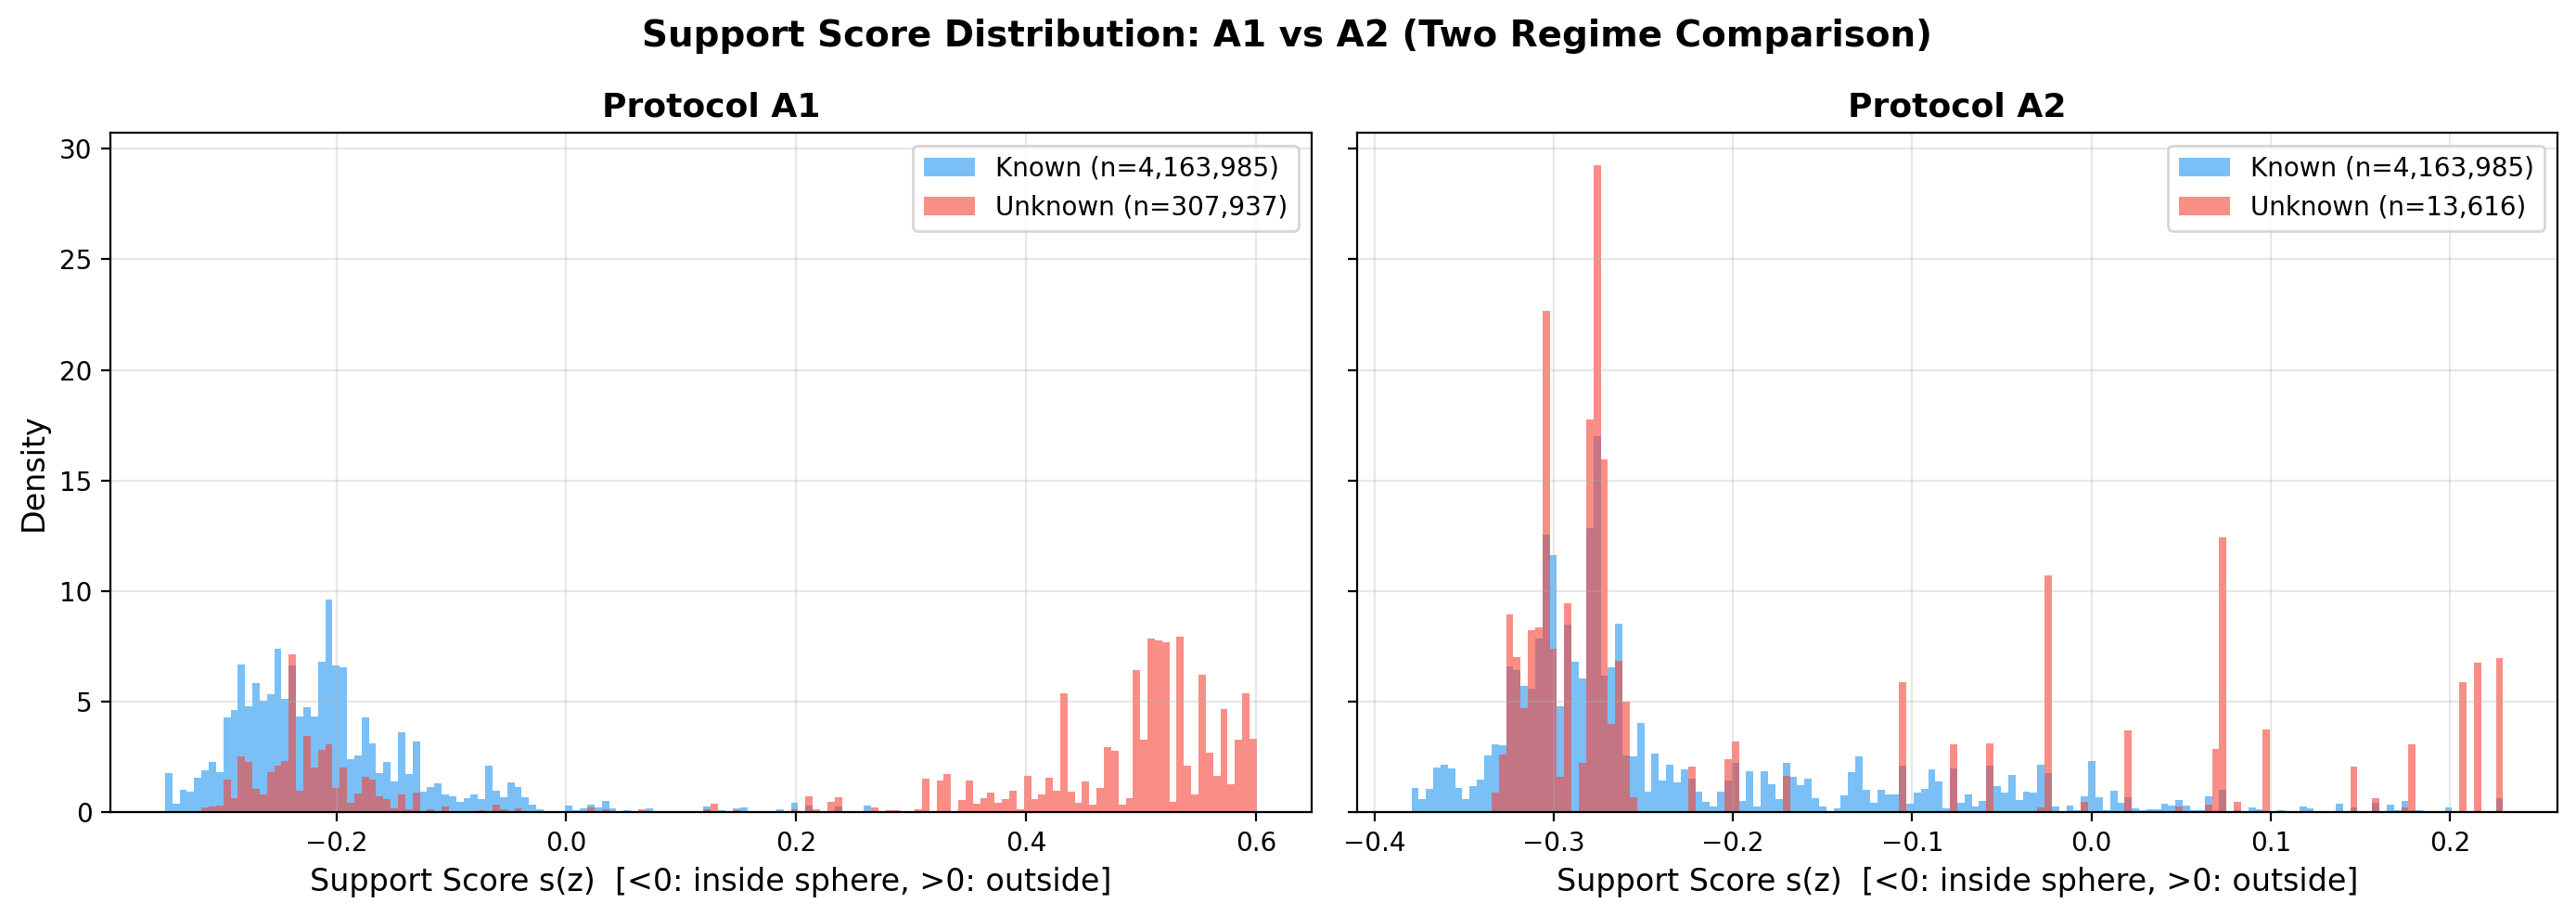
\includegraphics[width=\textwidth]{t1_support_a1_vs_a2.pdf}%
  }{%
    \IfFileExists{t1_support_a1_vs_a2.png}{%
      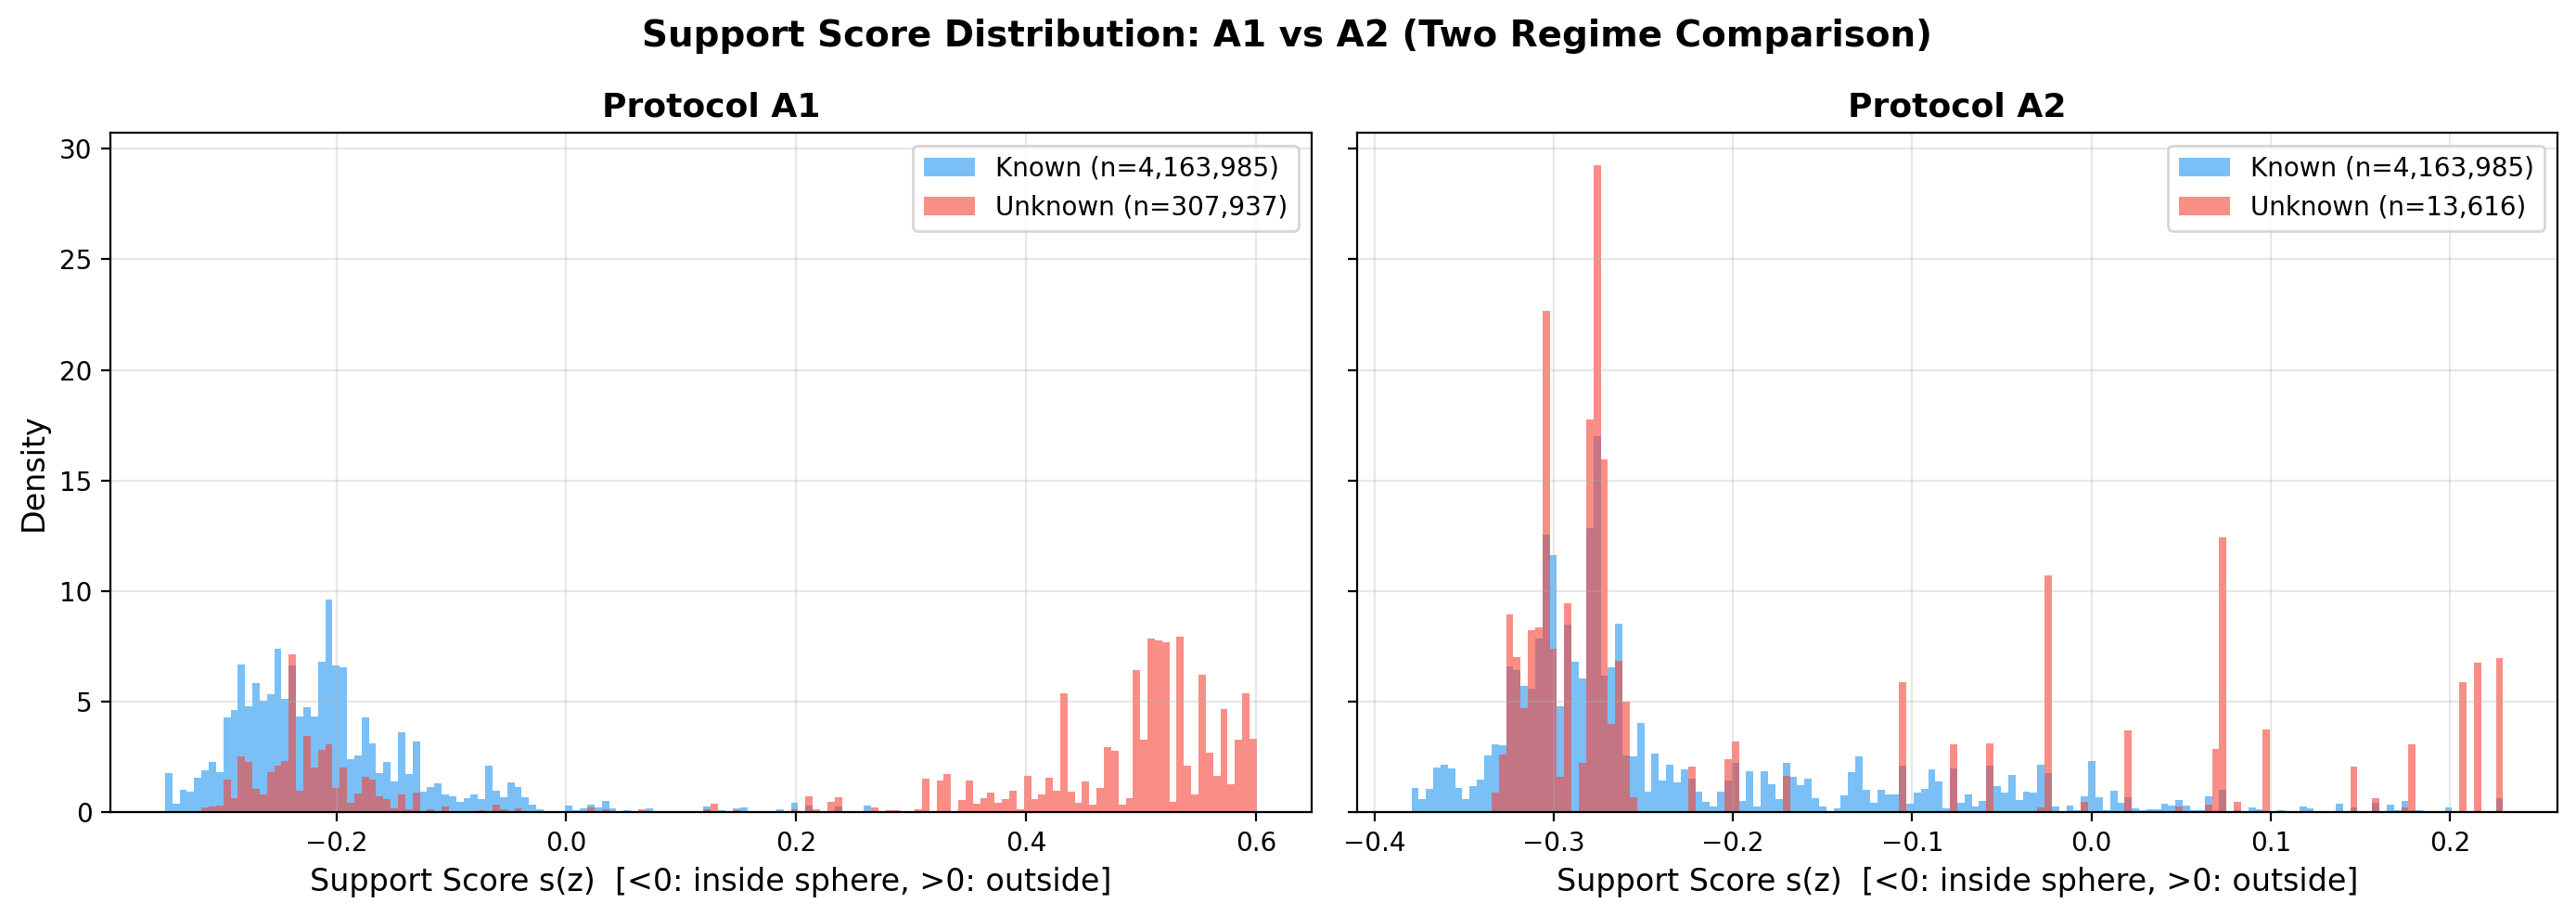
\includegraphics[width=\textwidth]{t1_support_a1_vs_a2.png}%
    }{%
      \fbox{\parbox{\textwidth}{\centering\vspace{3cm}Support score distribution comparison placeholder\vspace{3cm}}}%
    }%
  }
  \caption{Distribution comparison of support scores for known and unknown classes under A1 (left) and A2 (right). In A1, the support score distributions of known and unknown regions are clearly separated (support-deficit regime), whereas in A2 they overlap substantially (competitive-ambiguity regime), limiting global ranking quality.}
  \label{fig:supp_score_dist}
\end{figure*}

\subsection{A2 Retrieval Analysis}

To further interpret the gap between high AUROC and near-zero structured-abstention F1,
Table~\ref{tab:supp_retrieval} analyzes A2 ensemble ranking from a retrieval
perspective. Among foreground pixels in A2, the unknown prevalence is only 0.32\%.

\begin{table}[h]
\centering
\caption{Synapse A2 top-$r$\% retrieval analysis ranked by ensemble score. Lift denotes enrichment relative to a random baseline.}
\label{tab:supp_retrieval}
\begin{tabular}{lcccc}
\toprule
Budget & Precision & Recall & FPR & Lift \\
\midrule
top-0.1\% & $0.100$ & $0.031$ & $0.001$ & $30.8\times$ \\
top-0.3\% & $0.209$ & $0.193$ & $0.002$ & $64.3\times$ \\
top-0.5\% & $0.201$ & $0.310$ & $0.004$ & $62.0\times$ \\
top-1.0\% & $0.123$ & $0.380$ & $0.009$ & $38.0\times$ \\
\bottomrule
\end{tabular}
\end{table}

The ranking signal shows clear enrichment over chance, with lift reaching
$64.3\times$ at top-0.3\%. However, even at top-1\%, recall is only 0.380 and
precision is only 0.123. These results indicate that A2 detection signals carry
meaningful retrieval value, but this ranking quality remains insufficient to generate
high-quality structured abstention masks directly.

\section{Exploratory Mitigation of the Candidate Purity Bottleneck}

The main paper identifies candidate generation as the central bottleneck for A2
structured abstention. We therefore conducted exploratory experiments along two
pathways to better localize the failure mode.

\subsection{Pathway 1: Known-Exclusion Loss}

An intuitive hypothesis is that penalizing unknown responses in known-class regions
would improve purity. However, offline diagnosis reveals that the majority of
false-positive candidate pixels fall in background rather than known interiors, so this
design assumption does not align with the dominant error source. In our experiments,
the exclusion loss did not improve purity and instead degraded known-class performance.

\subsection{Pathway 2: Proposal-Conditioned Refinement}

The second pathway constructs proposals from an ensemble anomaly map and progressively
tests where the bottleneck resides.
First, the detection signal itself is not the primary problem: taking the top-0.3\%
foreground pixels and extracting connected components yields ensemble-proposal union IoU
of 0.153 and slice hit rate $\text{hit@IoU}{\geq}0.10=0.70$, both far above the current
unknown-slot candidates (0.005 and 0.02, respectively).
Second, a linear separability test on proposal tokens suggests that matched and
unmatched proposals are already well separated in feature space (linear probe
AUROC$=0.991$, centroid distance$=8.95$).
This narrows the unresolved problem to the conversion from separable proposal tokens to
pixel-level coherent masks.

\begin{table}[h]
\centering
\caption{Comparison of proposal-conditioned refinement variants against the ensemble proposal upper bound on Synapse A2.}
\label{tab:supp_e8}
\resizebox{\columnwidth}{!}{%
\begin{tabular}{lccc}
\toprule
Variant & Union IoU & Hit@IoU$\geq$0.10 & Comp Prec@IoU$\geq$0.10 \\
\midrule
E8 v1 (direct re-drawing)         & 0.039 & 0.080 & 0.048 \\
E8 v2 (residual refinement)       & 0.071 & 0.420 & 0.169 \\
E8 v3b (best variant)             & 0.073 & 0.440 & 0.172 \\
\midrule
Ensemble proposal upper bound ($r=0.3\%$) & 0.153 & 0.700 & 0.188 \\
\bottomrule
\end{tabular}
}%
\end{table}

Table~\ref{tab:supp_e8} shows that directly re-drawing masks is nearly ineffective.
Residual local refinement improves the result, but the best tested variant still
remains well below the proposal upper bound. Taken together, these exploratory results
reinforce the main-paper conclusion: stronger thresholding is not the missing ingredient;
the remaining challenge is a generation mechanism that can turn proposal-level
separability into pixel-level coherent masks.

\section{Additional Supporting Results}

\subsection{A2 ROC and PR Curves}

\begin{figure*}[!t]
  \centering
  \IfFileExists{t3_roc_curve_a2.pdf}{%
    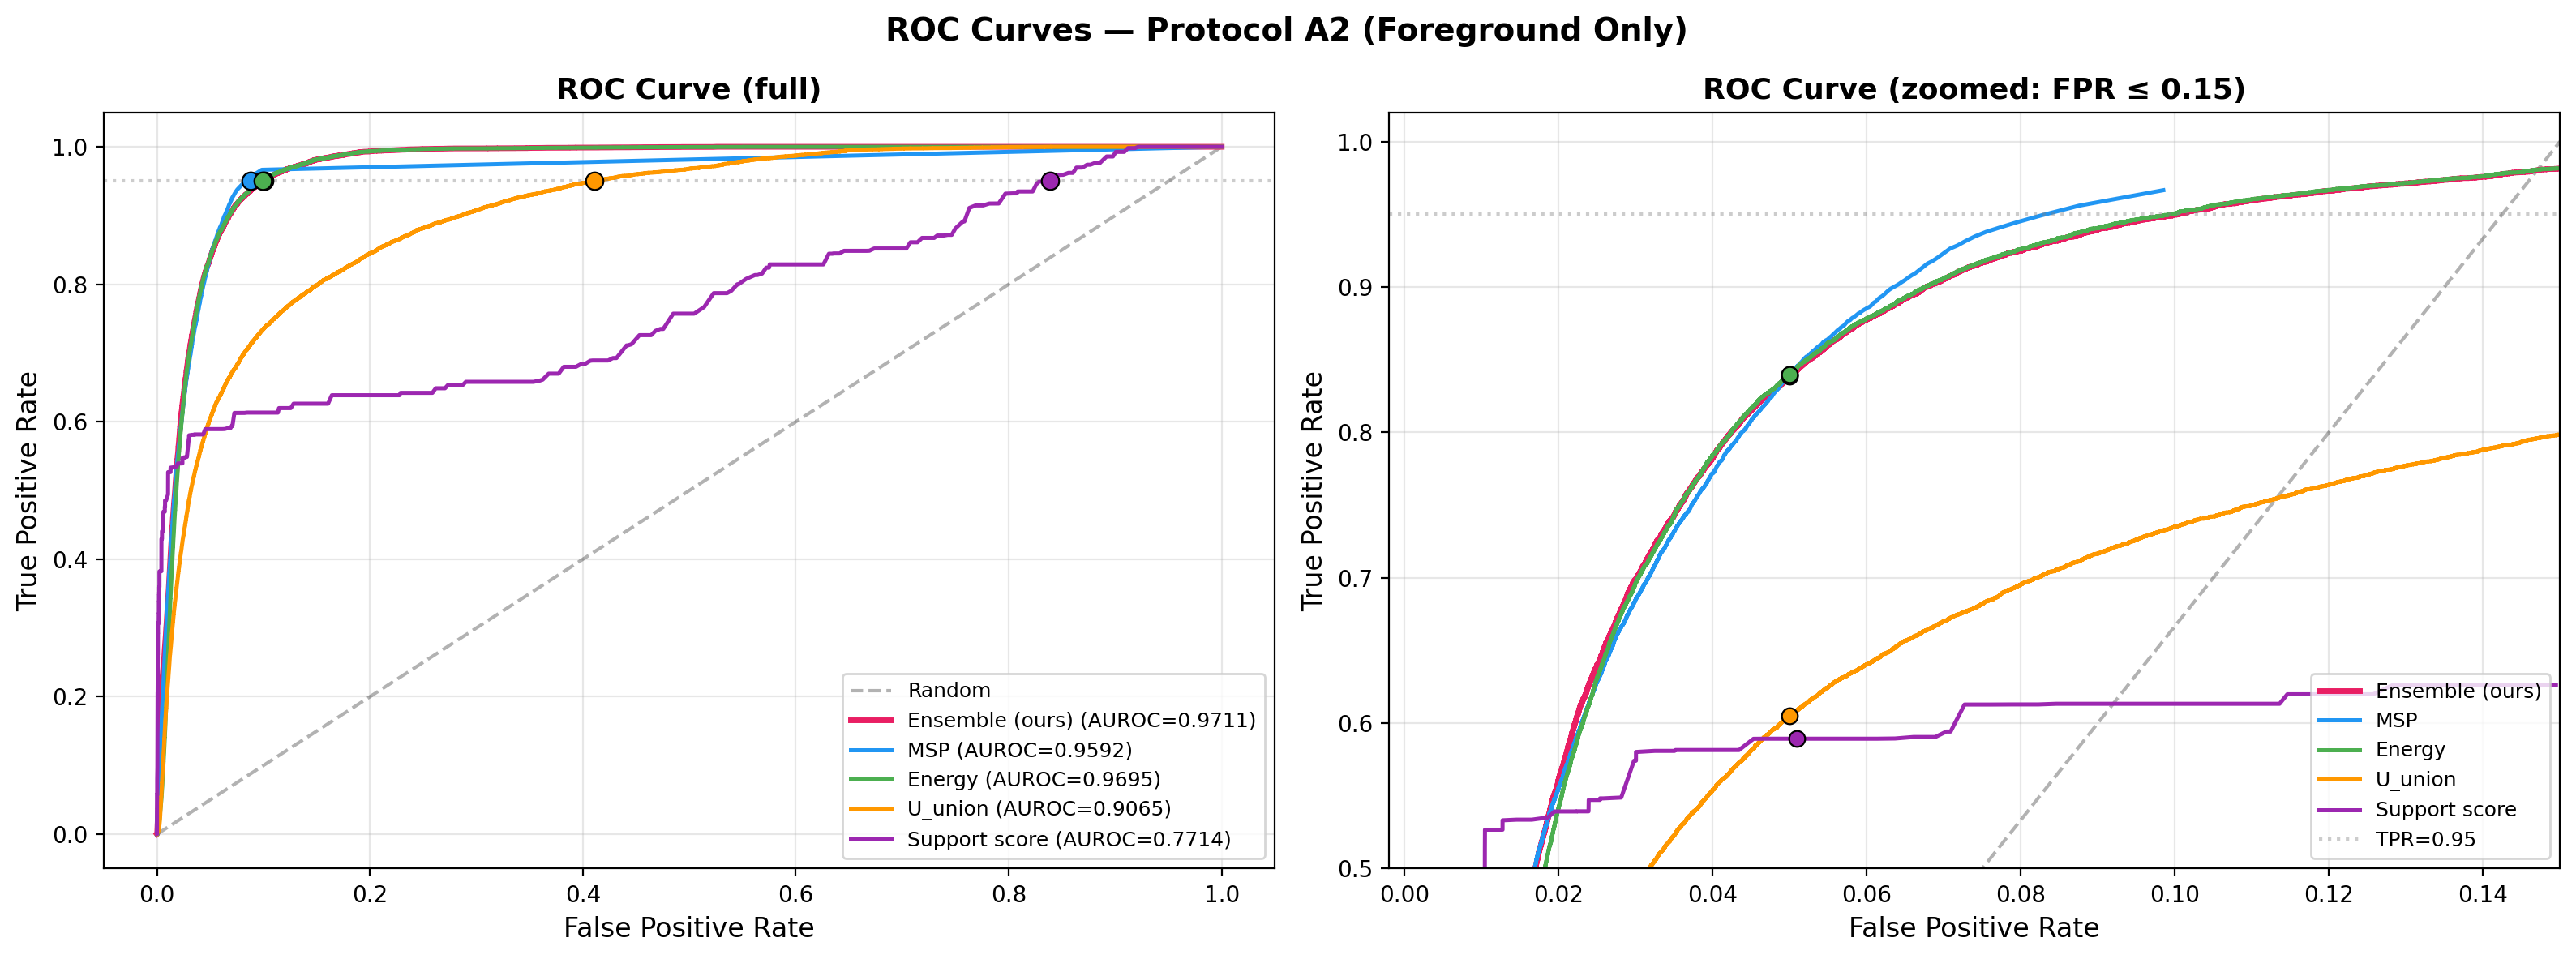
\includegraphics[width=\textwidth]{t3_roc_curve_a2.pdf}%
  }{%
    \IfFileExists{t3_roc_curve_a2.png}{%
      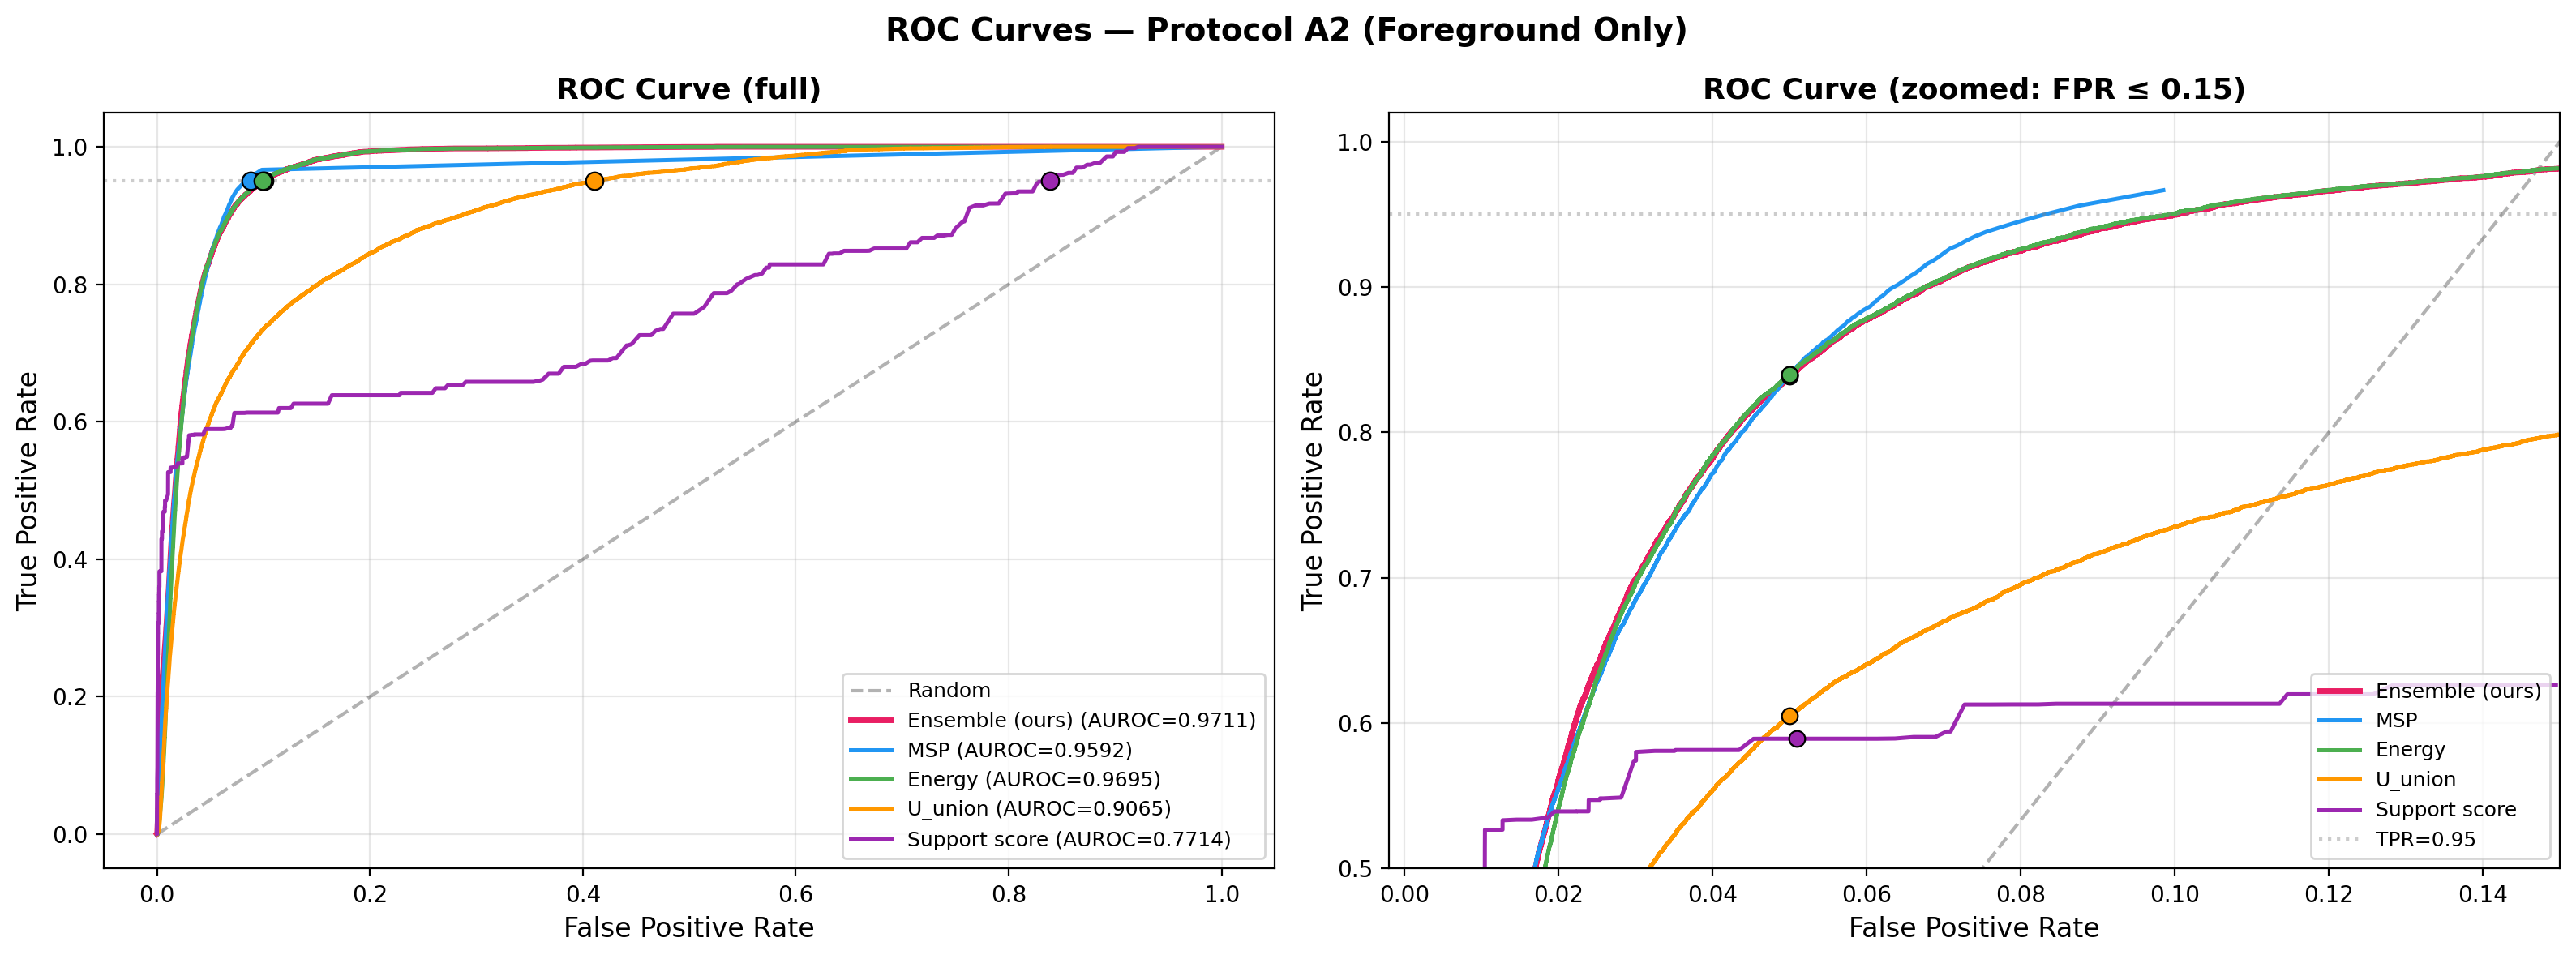
\includegraphics[width=\textwidth]{t3_roc_curve_a2.png}%
    }{%
      \fbox{\parbox{\textwidth}{\centering\vspace{4cm}ROC placeholder\vspace{4cm}}}%
    }%
  }
  \caption{ROC curves of different unknown detection signals under the Synapse A2 protocol (foreground pixels). Classification uncertainty signals substantially outperform the geometric support score in global ranking.}
  \label{fig:supp_a2_roc}
\end{figure*}

\begin{figure}[!t]
  \centering
  \IfFileExists{t3_pr_curve_a2.pdf}{%
    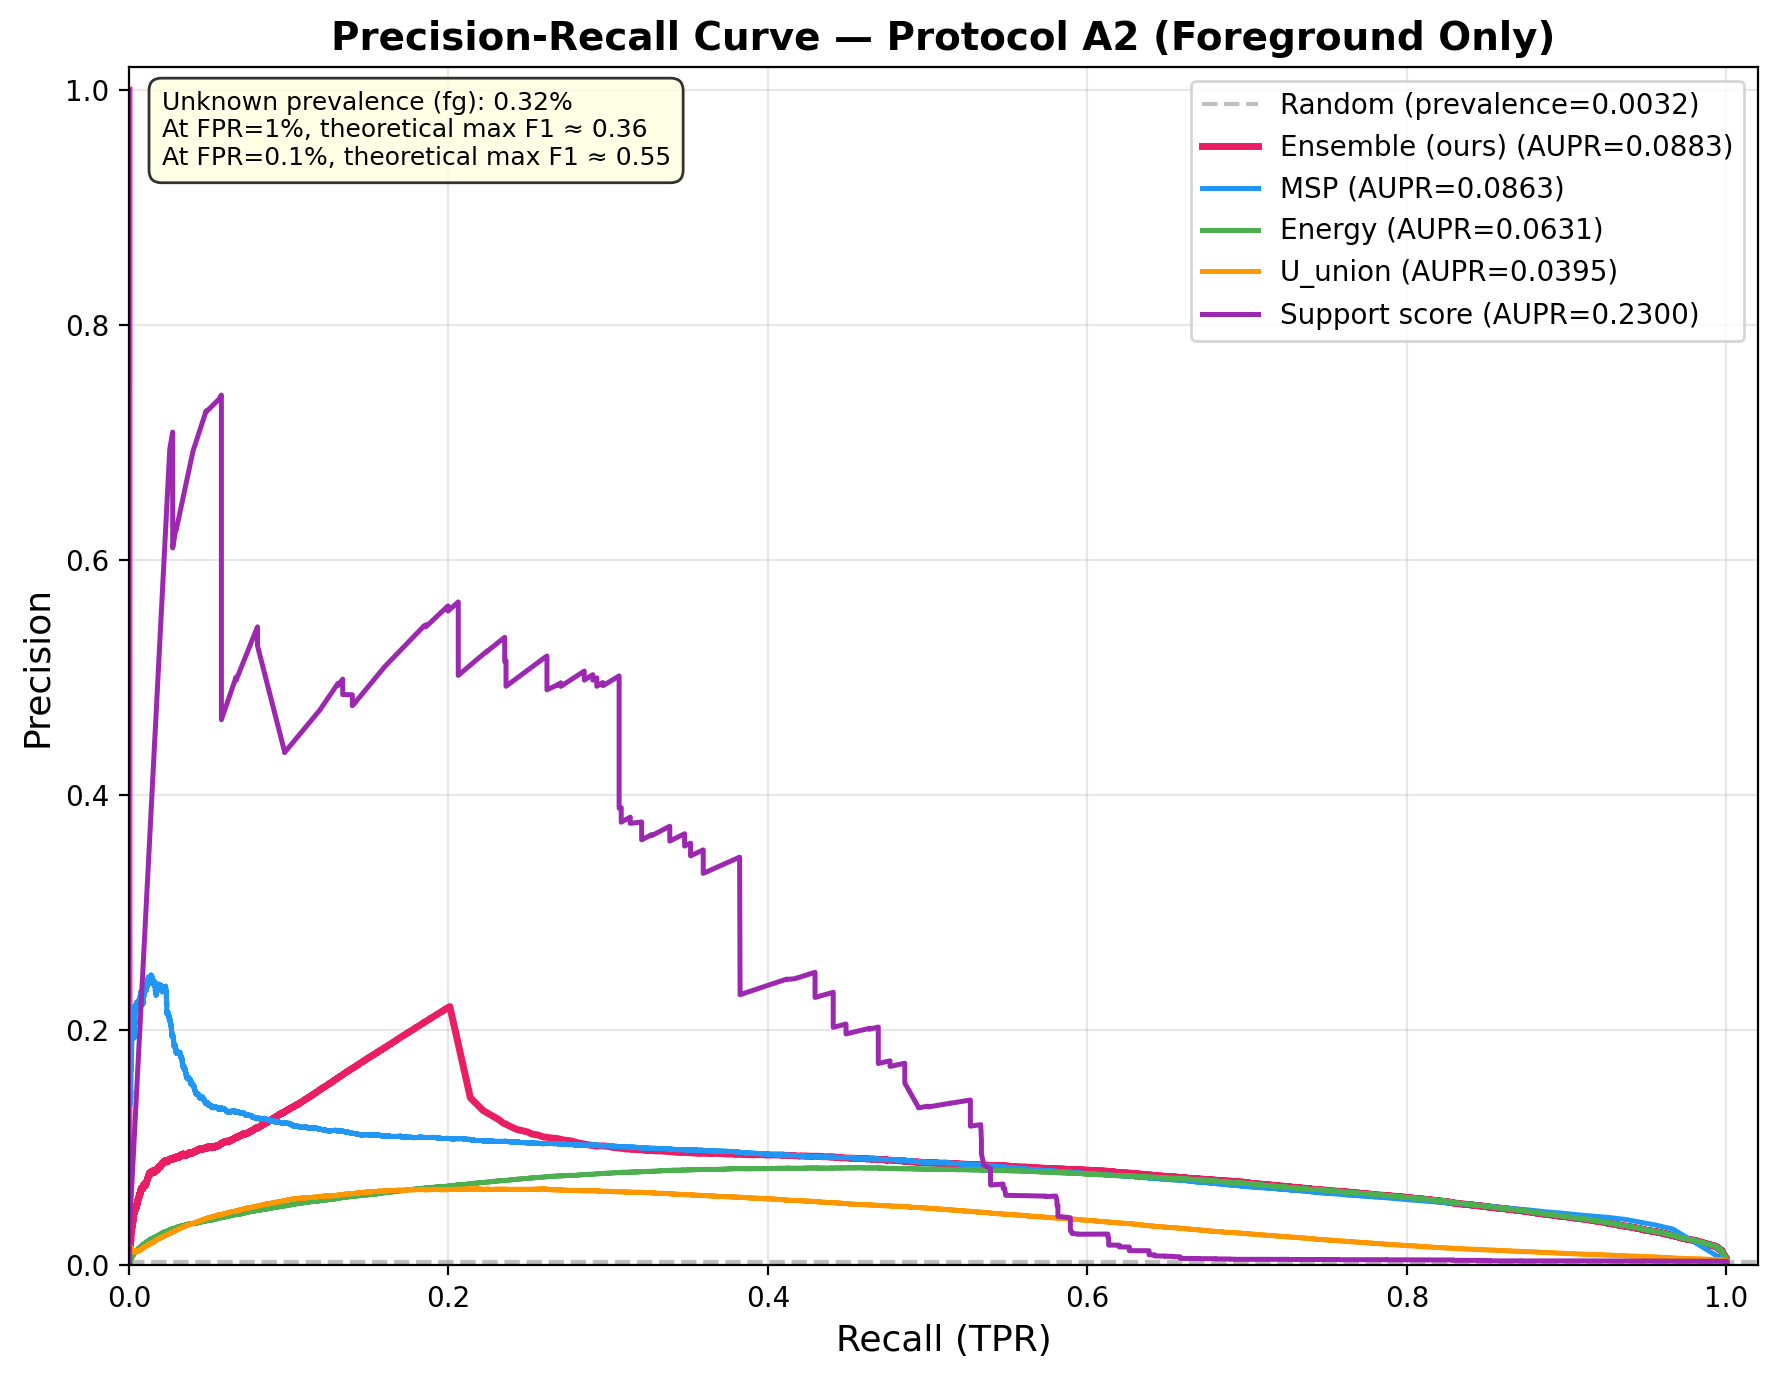
\includegraphics[width=\columnwidth]{t3_pr_curve_a2.pdf}%
  }{%
    \IfFileExists{t3_pr_curve_a2.png}{%
      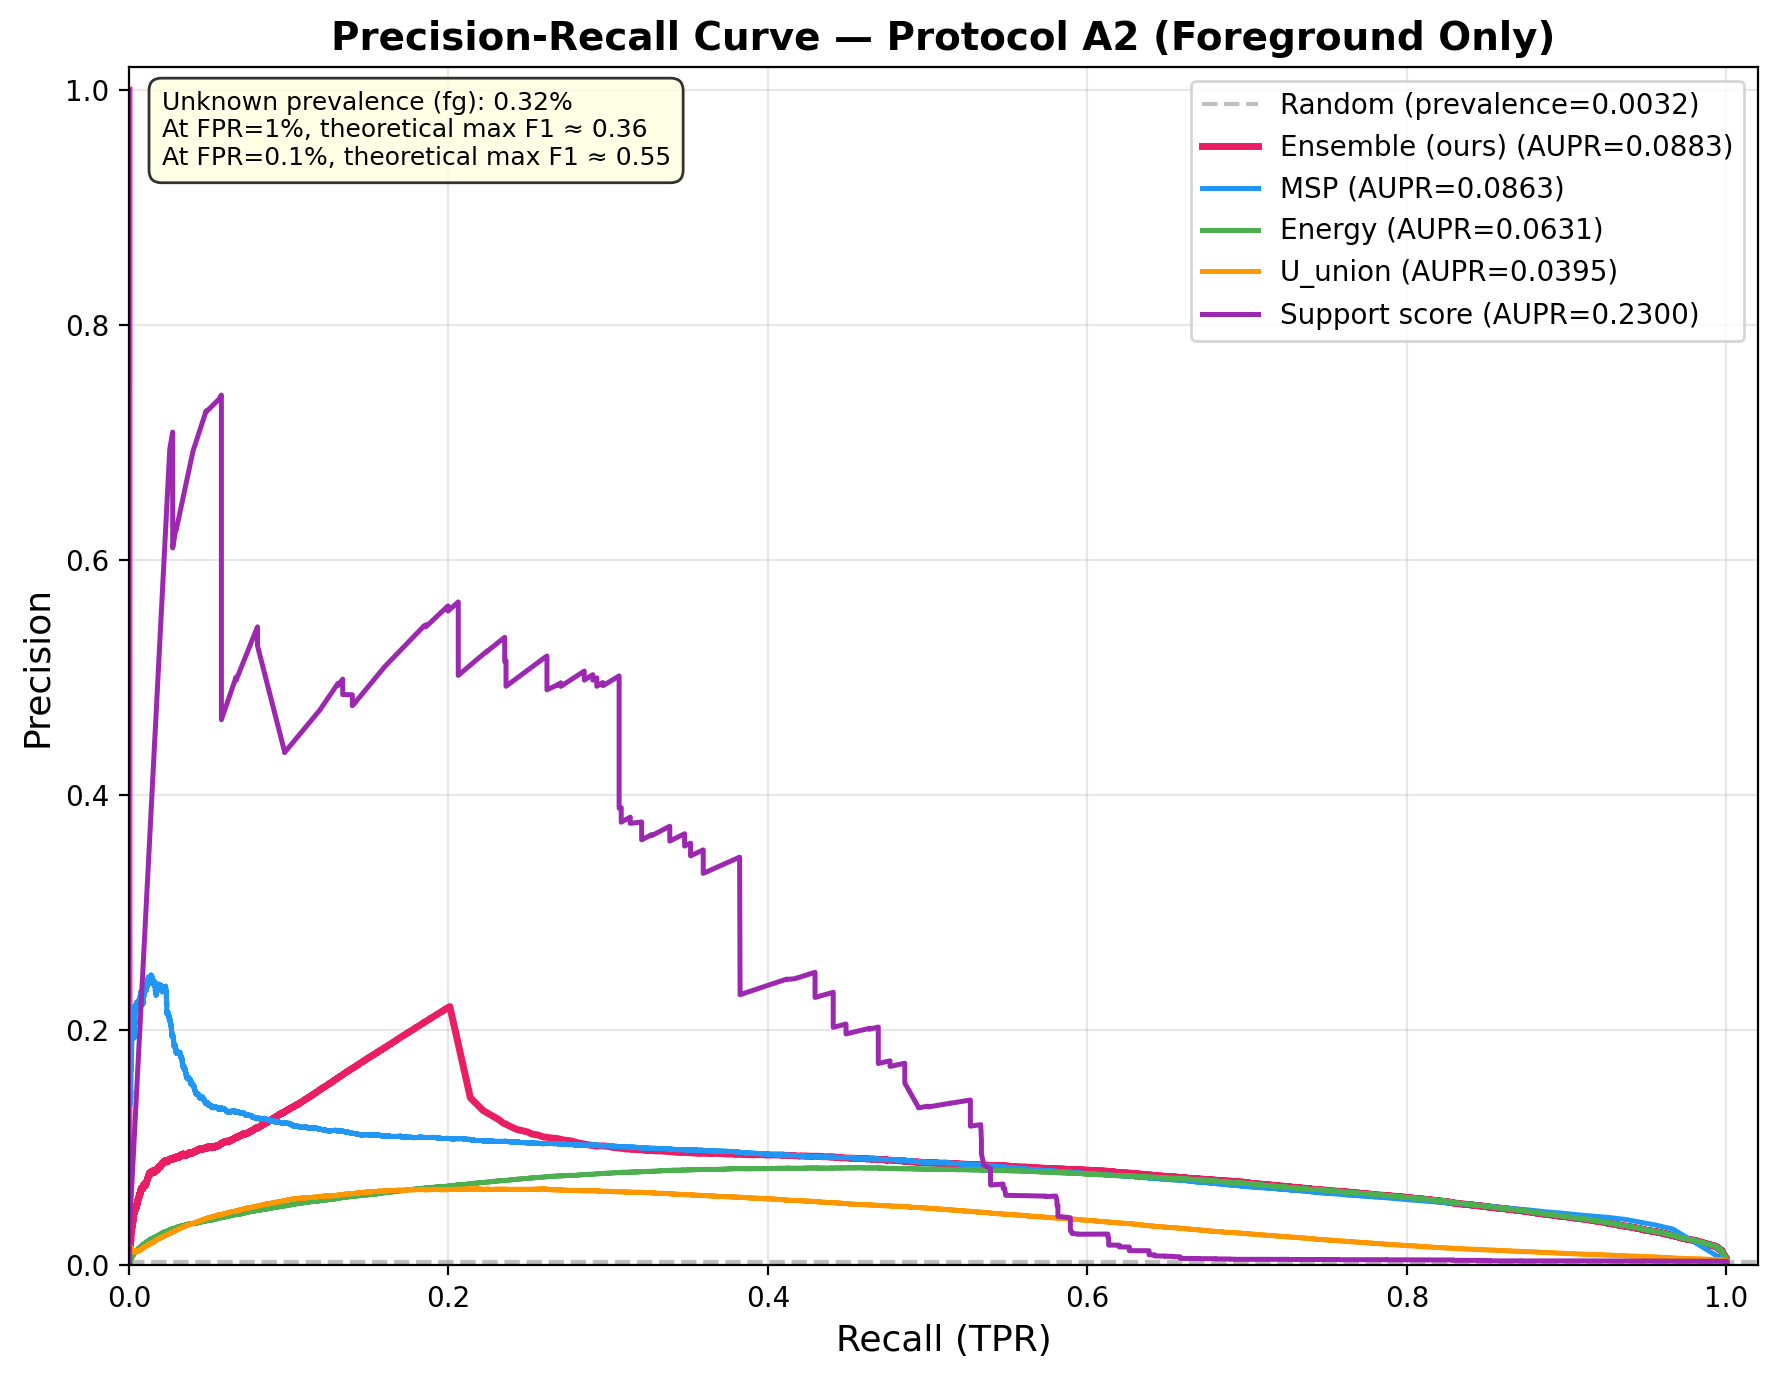
\includegraphics[width=\columnwidth]{t3_pr_curve_a2.png}%
    }{%
      \fbox{\parbox{\columnwidth}{\centering\vspace{4cm}PR placeholder\vspace{4cm}}}%
    }%
  }
  \caption{Precision--Recall curves of different unknown detection signals under the Synapse A2 protocol (foreground pixels). The support score retains a local advantage in the high-precision regime, but its overall AUPR is limited by weaker global ranking.}
  \label{fig:supp_a2_pr}
\end{figure}

\subsection{Split Robustness for the $M=0$ Ablation}

\begin{table}[h]
\centering
\caption{Alternative-split robustness check for the $M=0$ ablation on Synapse A1.}
\label{tab:supp_alt_split}
\begin{tabular}{llcc}
\toprule
Split & Setting & Known mIoU & Unknown F1 \\
\midrule
Original & $M=2$ (Support) & $0.811$ & $0.721$ \\
Original & $M=0$ (MSP) & $0.782$ & $0.070$ \\
\midrule
Alt-split & $M=2$ (Support) & $0.819$ & $0.787$ \\
Alt-split & $M=0$ (MSP) & $0.831$ & $0.043$ \\
\bottomrule
\end{tabular}
\end{table}

Under the alternative split, unknown F1 still collapses from 0.787 to 0.043 after
removing native unknown queries, corresponding to a 94.6\% reduction.
This mirrors the original-split result and shows that the main-paper $M=0$ conclusion
is not contingent on one particular class partition.

\subsection{Qualitative Comparison Between $M=2$ and $M=0$}

\begin{figure*}[!t]
  \centering
  \IfFileExists{t2_m2_vs_m0_grid.pdf}{%
    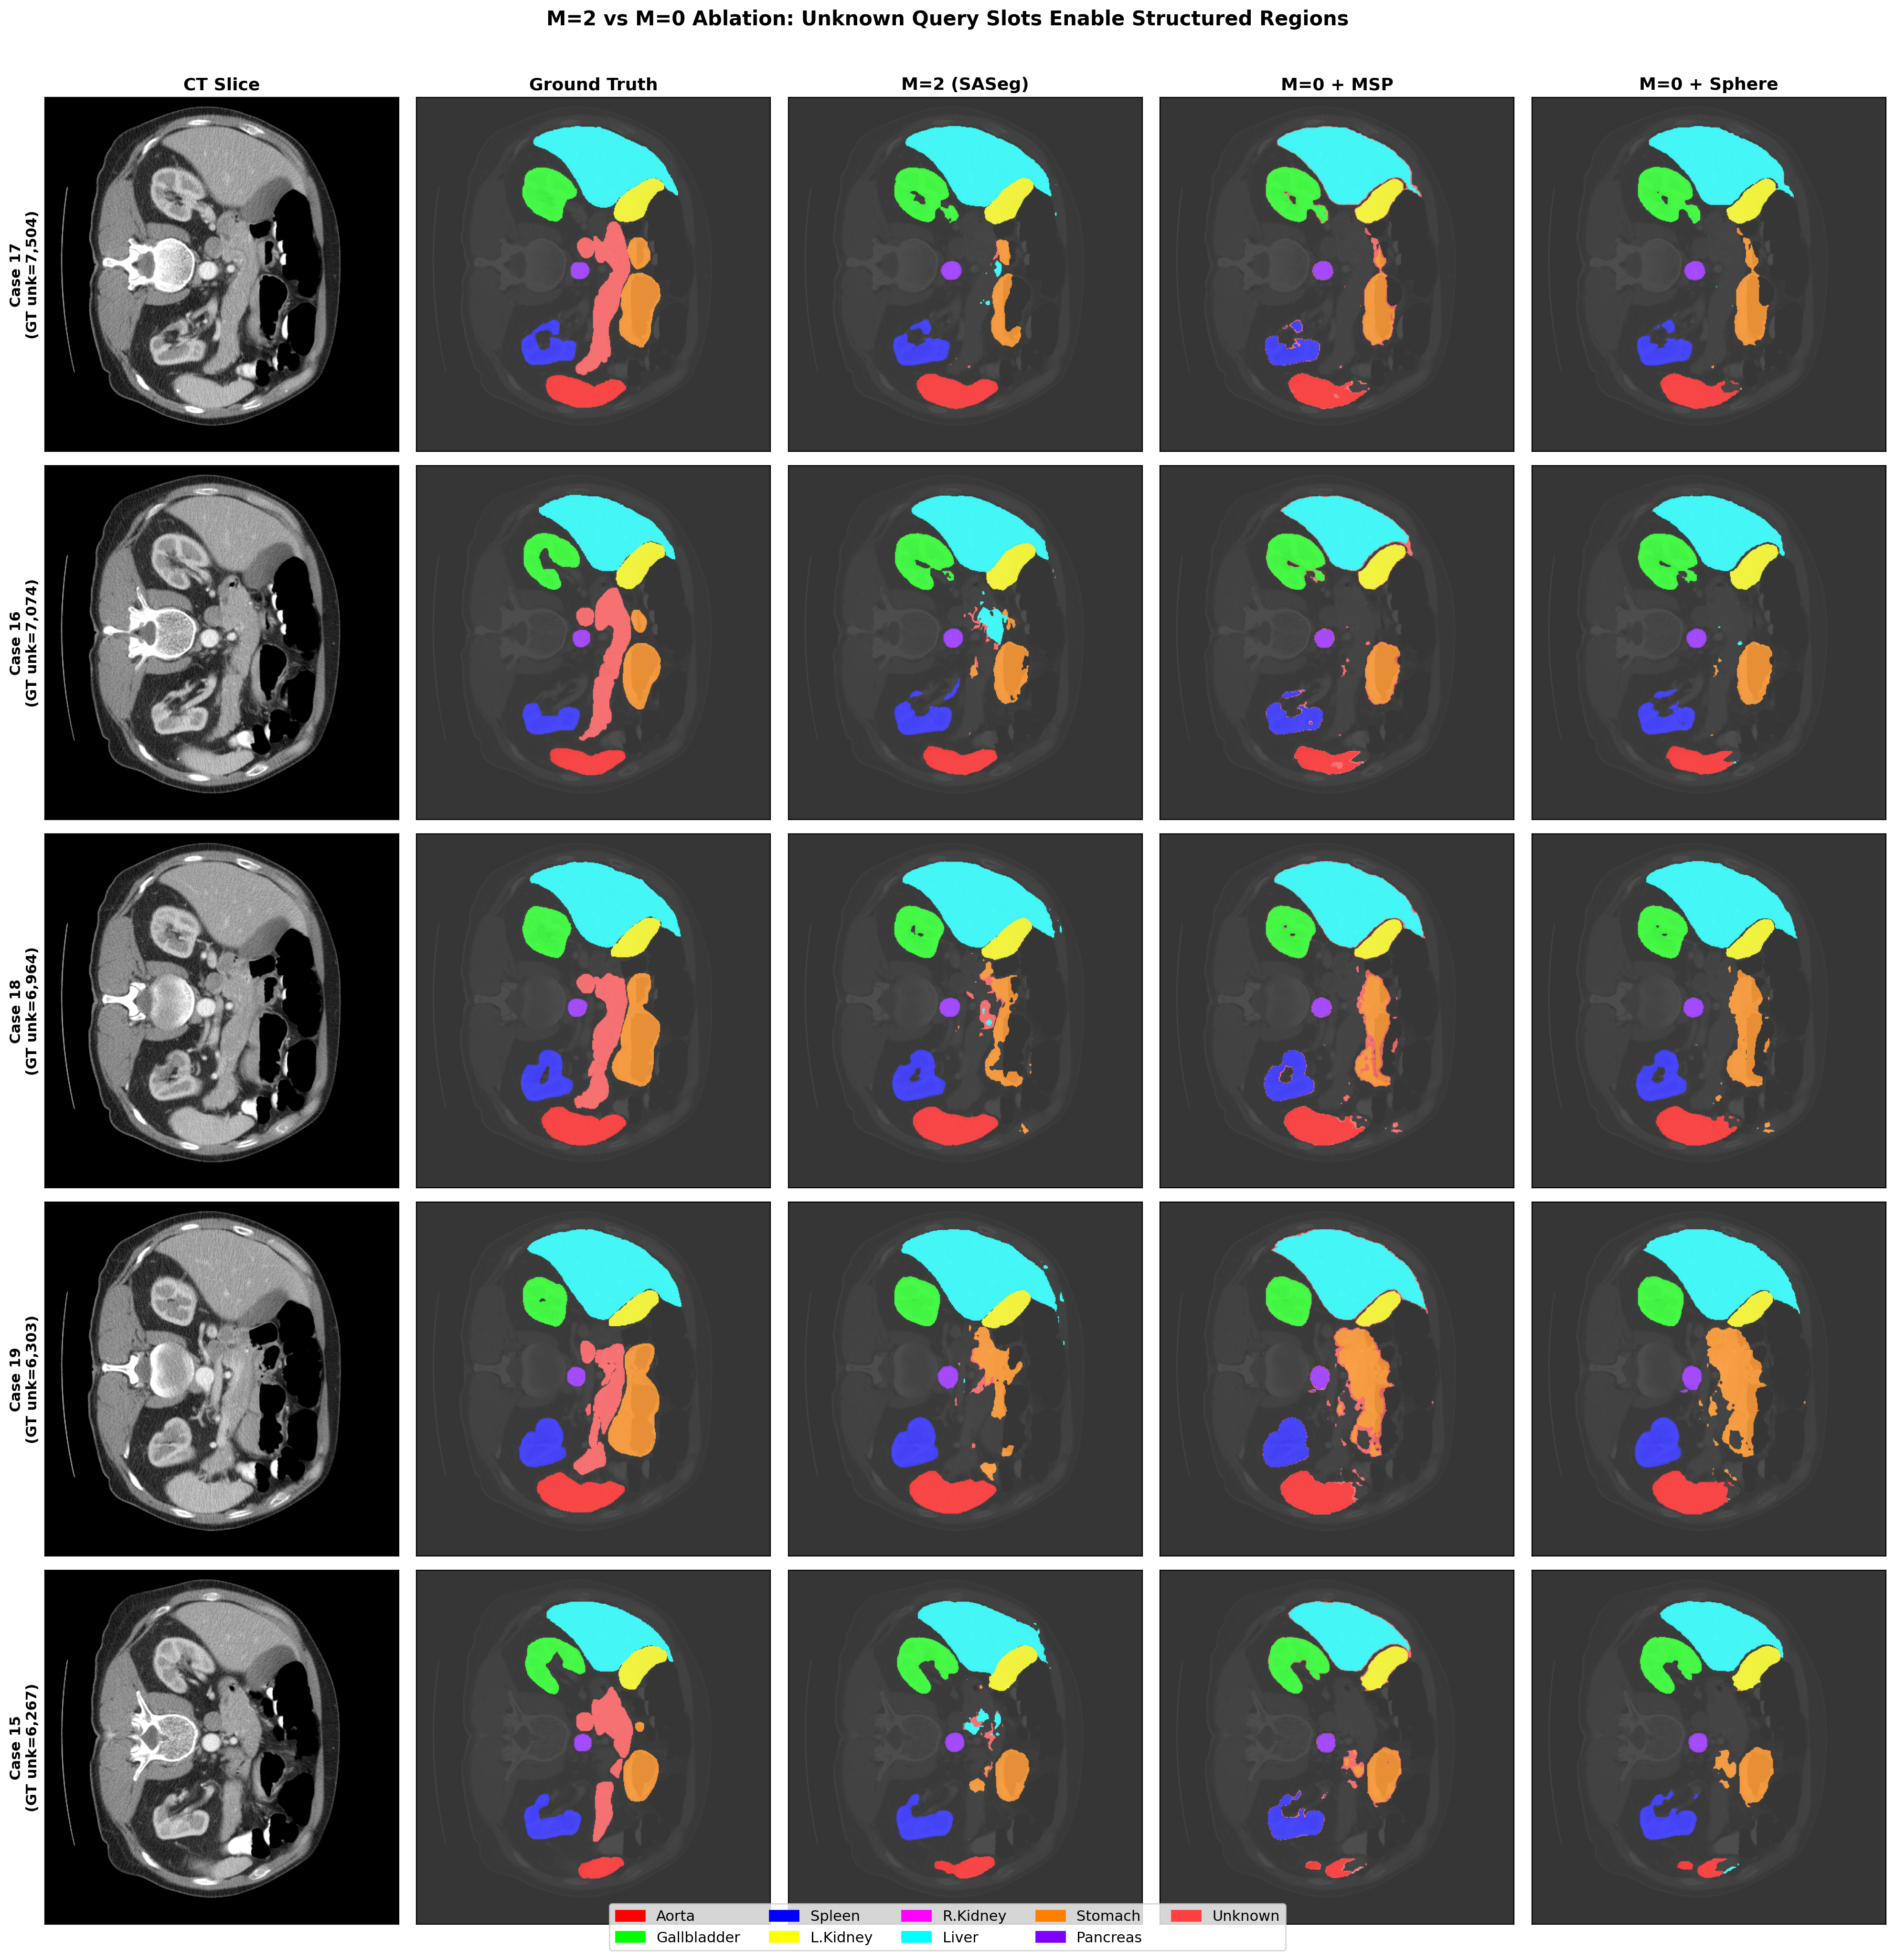
\includegraphics[width=\textwidth]{t2_m2_vs_m0_grid.pdf}%
  }{%
    \IfFileExists{t2_m2_vs_m0_grid.png}{%
      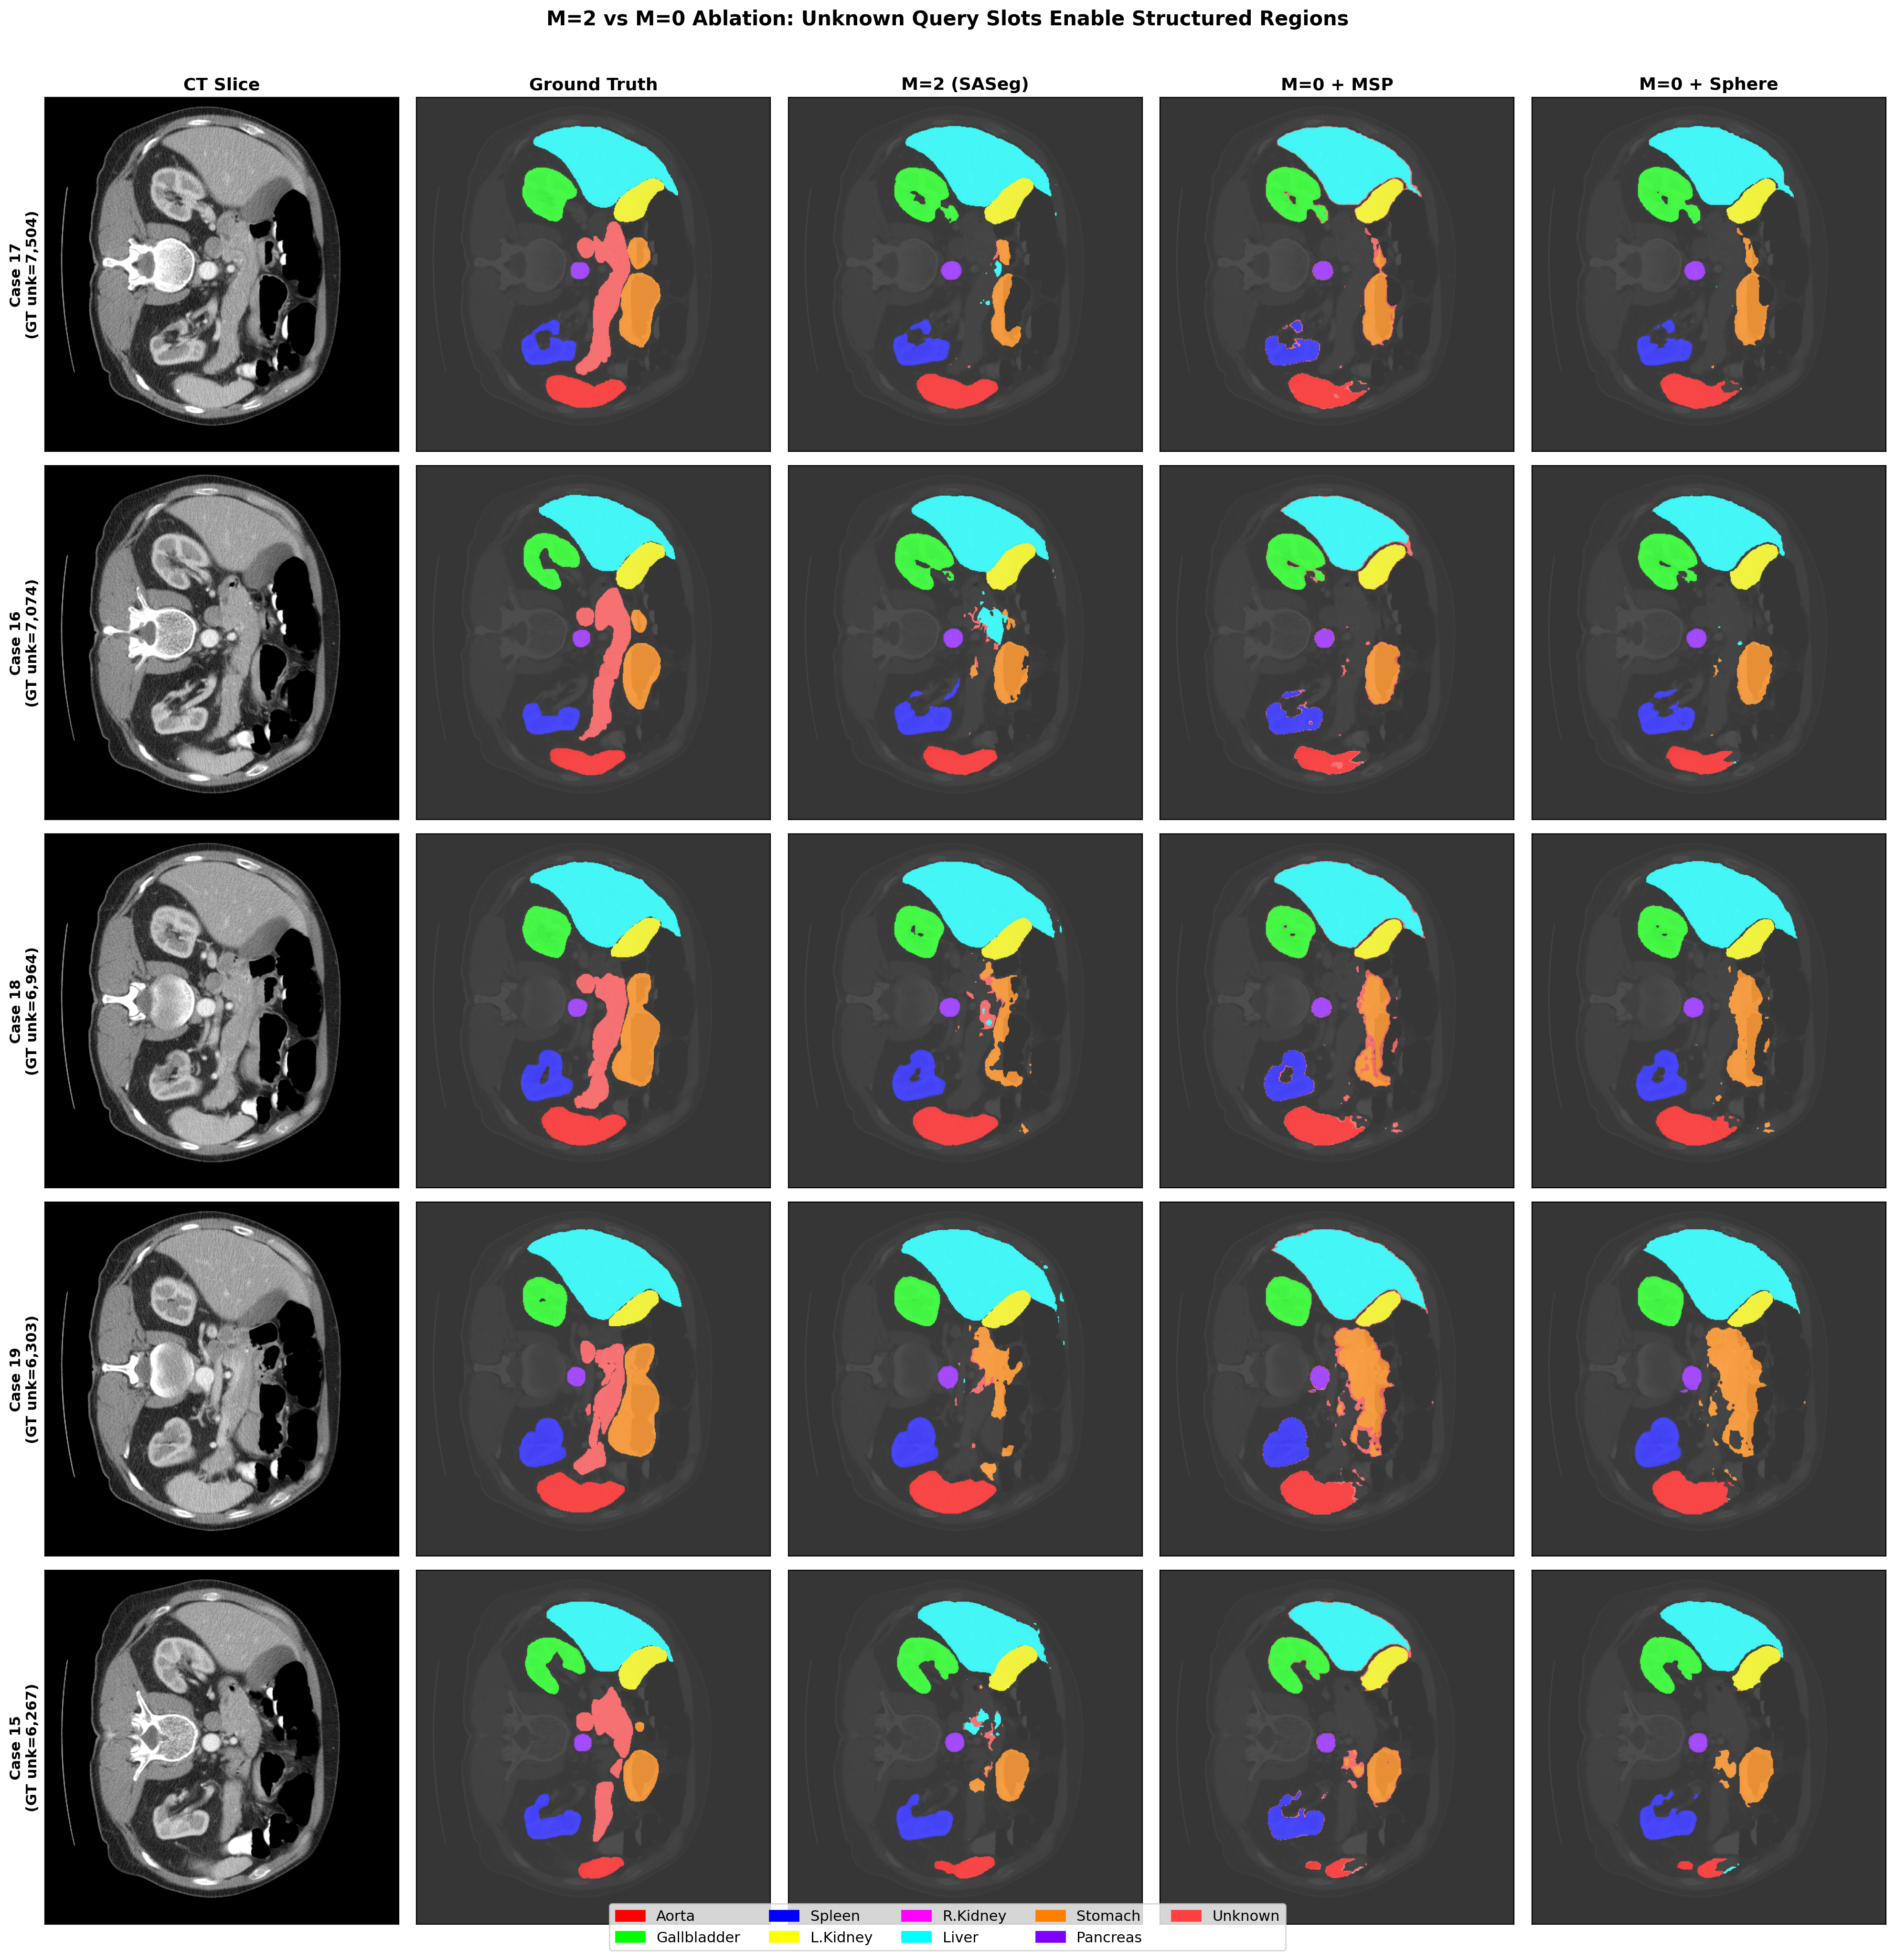
\includegraphics[width=\textwidth]{t2_m2_vs_m0_grid.png}%
    }{%
      \fbox{\parbox{\textwidth}{\centering\vspace{4cm}$M=2$ vs $M=0$ qualitative comparison placeholder\vspace{4cm}}}%
    }%
  }
  \caption{Qualitative comparison of $M=2$ (top) and $M=0$ (bottom) on Synapse A1. The $M=2$ model produces spatially coherent unknown masks via native unknown queries, whereas the post-hoc unknown determination of the $M=0$ model is fragmented and fails to form meaningful abstention regions.}
  \label{fig:supp_m0_vis}
\end{figure*}

\clearpage
\begin{thebibliography}{1}

\bibitem{everingham2010pascal}
M. Everingham, L. Van~Gool, C.~K.~I. Williams, J. Winn, and A. Zisserman,
``The {PASCAL} visual object classes ({VOC}) challenge,''
\emph{Int. J. Comput. Vis.}, vol.~88, no.~2, pp. 303--338, 2010.

\bibitem{cordts2016cityscapes}
M. Cordts, M. Omran, S. Ramos, T. Rehfeld, M. Enzweiler, R. Benenson,
U. Franke, S. Roth, and B. Schiele,
``The {Cityscapes} dataset for semantic urban scene understanding,''
in \emph{Proc. IEEE Conf. Comput. Vis. Pattern Recognit.}, 2016, pp. 3213--3223.

\end{thebibliography}

\end{document}
